\documentclass[a4paper,11pt]{article}

\usepackage[nottoc, notlof, notlot]{tocbibind}
\usepackage[sort,nocompress]{cite}
%\usepackage[margin=0.8in]{geometry}
\usepackage[hmargin=2.5cm,vmargin=2.5cm]{geometry}
\usepackage[francais]{babel}
\usepackage[utf8]{inputenc}
\usepackage{algpseudocode}
\usepackage[cyr]{aeguill}
\usepackage{lingmacros}
\usepackage{algorithm}
\usepackage{listings}
\usepackage{graphicx}
\usepackage{newclude}
\usepackage{booktabs}
\usepackage{rotating}
\usepackage{verbatim}
\usepackage{newclude}
\usepackage{multicol}
\usepackage{stmaryrd}
\usepackage{multirow}
\usepackage{amsmath}
\usepackage{xspace}
\usepackage{xcolor}
\usepackage{url}

%%%%%%%%%%%%%%%%%%%%%%%%%%%%%%%%
%             TODOs            %
%%%%%%%%%%%%%%%%%%%%%%%%%%%%%%%%
% [ ] = à faire
% [?] = fait mais à valider
% [X] = fait et validé
%%%%%%%%
% [ ] Faire Résumé
% [ ] Faire Introduction
% [ ] Faire la description des quatre stratégies
% [ ] Faire la description générale des expériences
% [ ] Faire le plan d'expérience pour un débris
% [ ] Faire l'analyse des résultats pour l'expérience à un débris
% [ ] Faire le plan d'expérience pour 100 débris uniformément répartis
% [ ] Faire l'analyse des résultats pour l'expérience à 100 débris uniformément répartis
% [ ] Faire le plan d'expérience pour 100 débris répartis en 10 clusters (écart-type 3)
% [ ] Faire l'analyse des résultats pour l'expérience à 100 débris répartis en 10 clusters (écart-type 3)
% [ ] Conclusion
%%%%%%%% FINALISATION (à faire qu'à la fin)
% [ ] Mettre en forme
%%%%%%%%%%%%%%%%%%%%%%%%%%%%%%%%  

\begin{document}
	
\title{Intelligence artificielle bio-inspirée \\ Compte-rendu}
\author{Adrien Castex\\Polytech Informatique\\et Master Recherche IA\\\texttt{\small adrien.castex@etu.univ-lyon1.fr} \and Alexandre Galdeano\\Polytech Informatique\\et Master Recherche IA\\\texttt{\small alexandre.galdeano@etu.univ-lyon1.fr}}
%\date{05/02/2016}
\maketitle

\begin{abstract}



\end{abstract}

\tableofcontents
\listoffigures
\thispagestyle{empty}
\clearpage

\setcounter{page}{1}
\begin{multicols*}{2}
%!TEX root = ../Compte-rendu.tex
\section{Les quatre stratégies}
\subsection{Brownien}
\subsection{\'{E}quiprobable}
\subsection{Custom}
\subsection{Lévy}
%!TEX root = ../Compte-rendu.tex
\section{Caractéristiques communes aux trois expériences}
\subsection{Environnement}
\subsection{Variable mesurée}

\section{Un seul débris}
%!TEX root = ../../Compte-rendu.tex
%\subsection{Description}
La seconde comparaison sera faite avec cent débris répartis uniformément.
%!TEX root = ../../Compte-rendu.tex


\begin{figure}[H]
	\begin{center}
		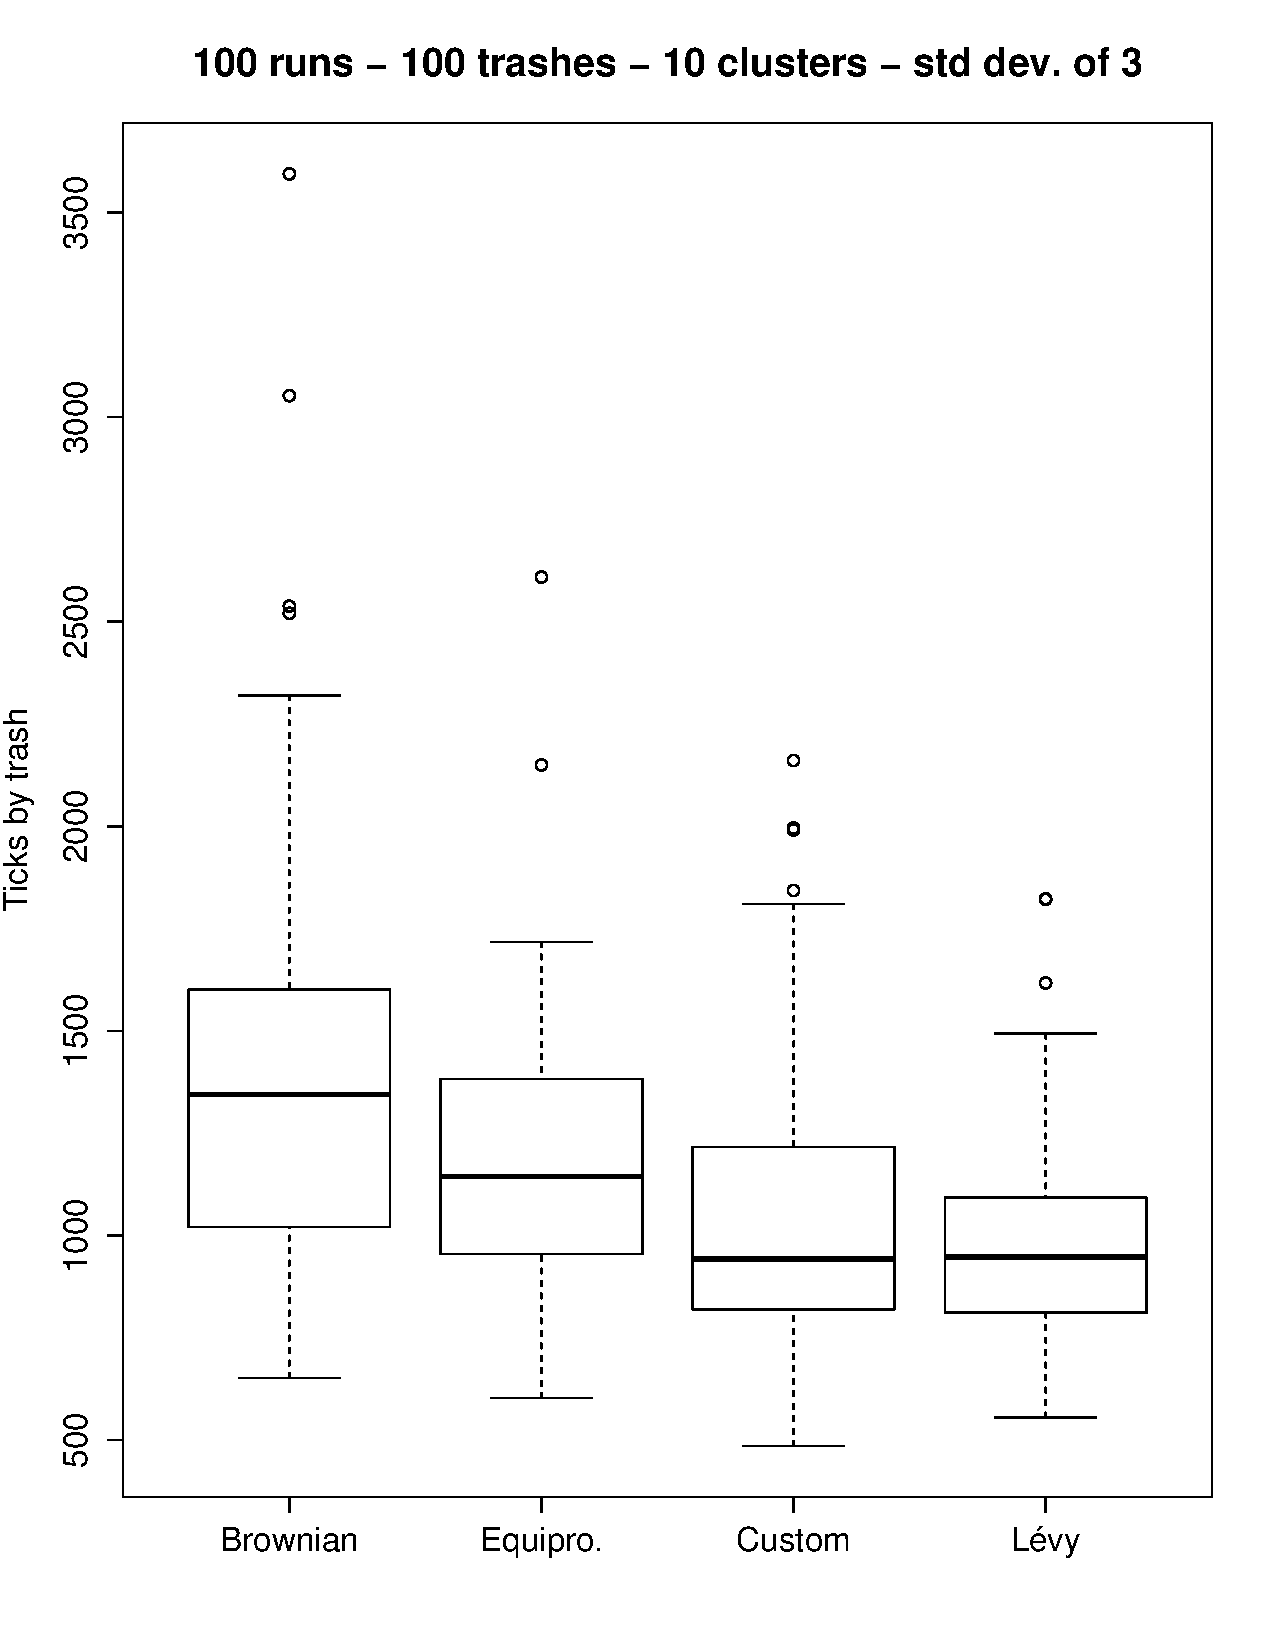
\includegraphics[height=10cm]{diagrams/100Tr10Clts_all.pdf}
		\caption{Résultat des mesures pour 100 débris distribué en 10 clusters (écart-type 3)}
		\label{fig:100Trashes_10Clusters}
	\end{center}
\end{figure}

Nous avons pour les différentes stratégies les statistiques suivantes :

\begin{figure}[H]
	\begin{center}
		\begin{tabular}{| c || c | c | c | c | }
			\hline
			&Brown.&Equi.&Custom&Lévy \\
			\hline
			\hline
			md&1344&1144&942&947\\
			mean&1388&1187&1053&984\\
			min & 652 & 602 & 485 & 555 \\
			max & 3595 & 2609 & 2161 & 1823 \\
			sd&491&318&344&256\\
			p-val&$\ll 5\%$&$\ll 5\%$&$\ll 5\%$&$\ll 5\%$\\
			\hline
		\end{tabular}
		\caption{Statistiques pour 100 débris distribué en 10 clusters (écart-type 3)}
	\end{center}
\end{figure}


Nous pouvons constater que la stratégie Custom a une médiane très
légèrement meilleure à la stratégie Lévy, néanmoins cette première
est moins fiable, c'est à dire que celle-ci a plus de chance de produire
des résultats bien moins bons que le Lévy.

Nous pouvons aussi voir que la stratégie Custom perd en fiabilité
alors que la stratégie Equiprobable, elle, en gagne.

\section{Cent débris uniformément répartis}
%!TEX root = ../../Compte-rendu.tex
%\subsection{Description}
La seconde comparaison sera faite avec cent débris répartis uniformément.
%!TEX root = ../../Compte-rendu.tex


\begin{figure}[H]
	\begin{center}
		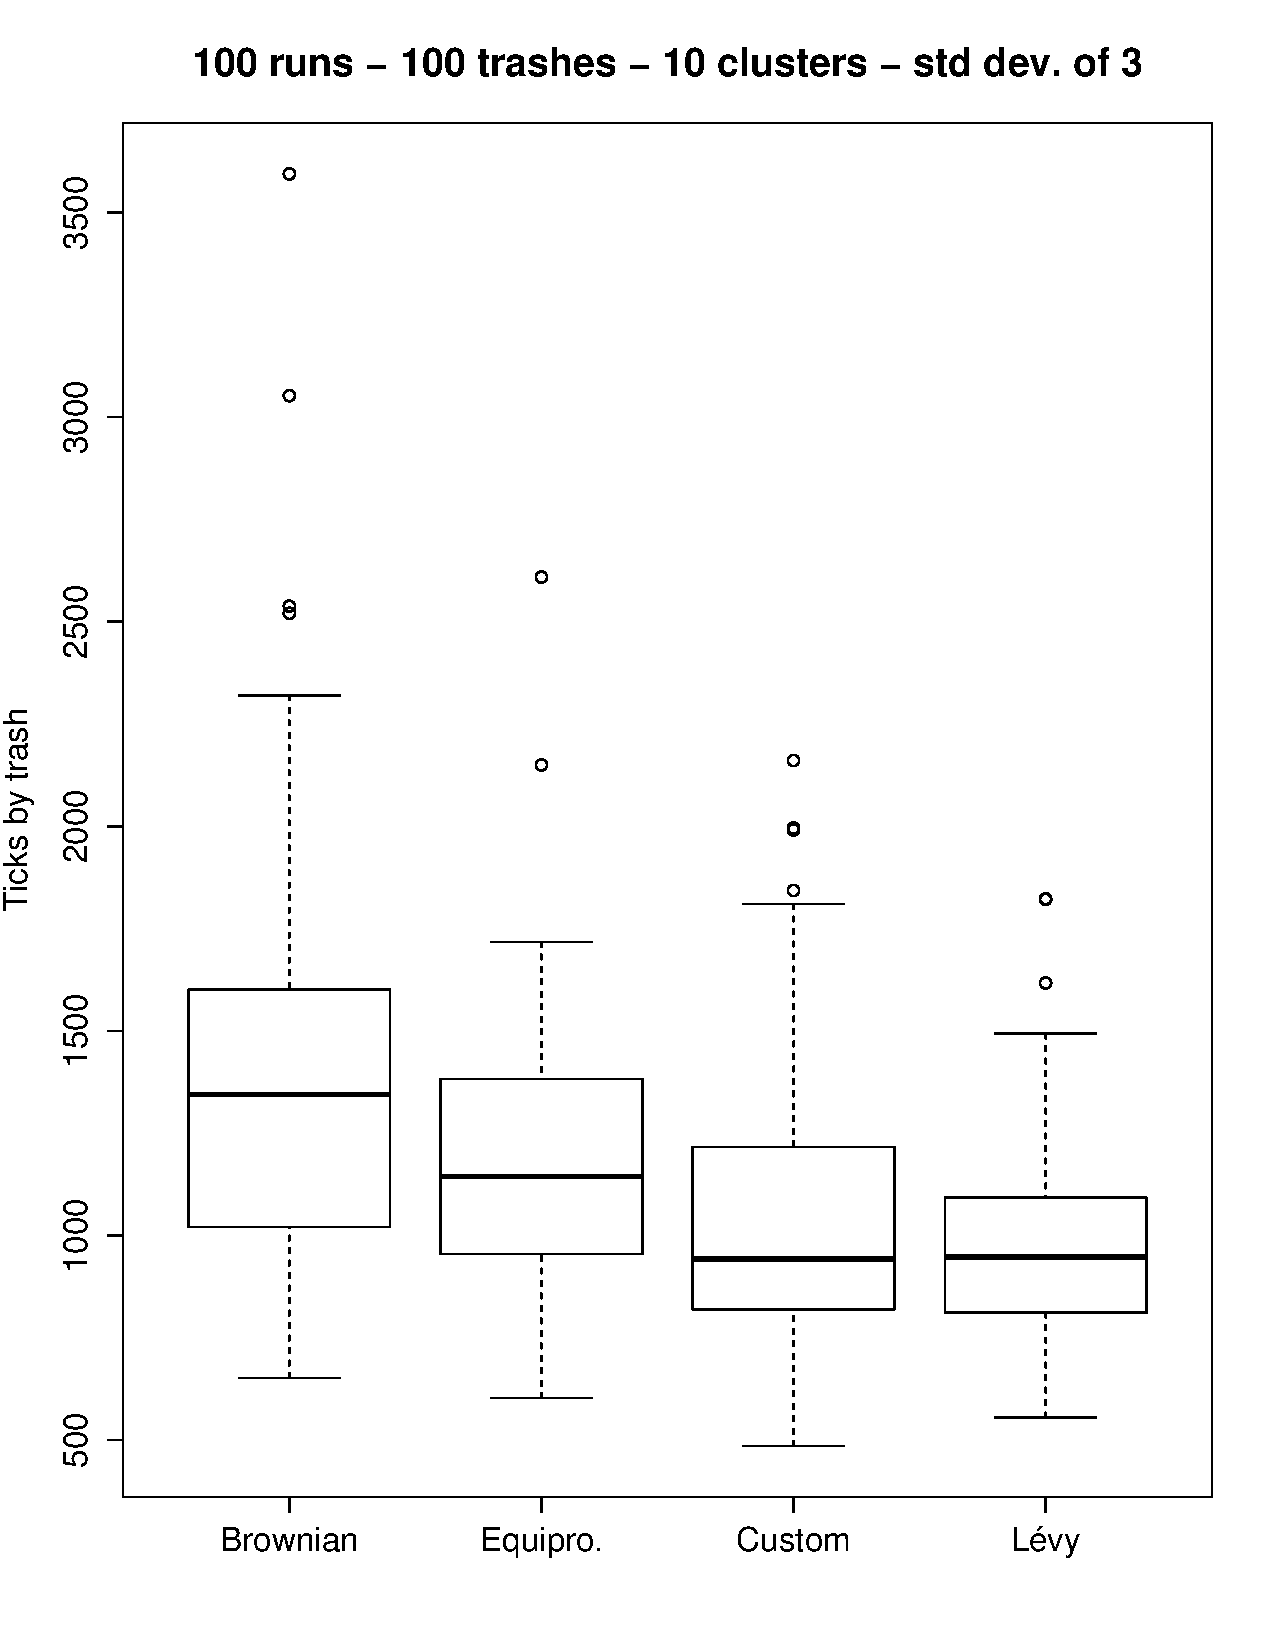
\includegraphics[height=10cm]{diagrams/100Tr10Clts_all.pdf}
		\caption{Résultat des mesures pour 100 débris distribué en 10 clusters (écart-type 3)}
		\label{fig:100Trashes_10Clusters}
	\end{center}
\end{figure}

Nous avons pour les différentes stratégies les statistiques suivantes :

\begin{figure}[H]
	\begin{center}
		\begin{tabular}{| c || c | c | c | c | }
			\hline
			&Brown.&Equi.&Custom&Lévy \\
			\hline
			\hline
			md&1344&1144&942&947\\
			mean&1388&1187&1053&984\\
			min & 652 & 602 & 485 & 555 \\
			max & 3595 & 2609 & 2161 & 1823 \\
			sd&491&318&344&256\\
			p-val&$\ll 5\%$&$\ll 5\%$&$\ll 5\%$&$\ll 5\%$\\
			\hline
		\end{tabular}
		\caption{Statistiques pour 100 débris distribué en 10 clusters (écart-type 3)}
	\end{center}
\end{figure}


Nous pouvons constater que la stratégie Custom a une médiane très
légèrement meilleure à la stratégie Lévy, néanmoins cette première
est moins fiable, c'est à dire que celle-ci a plus de chance de produire
des résultats bien moins bons que le Lévy.

Nous pouvons aussi voir que la stratégie Custom perd en fiabilité
alors que la stratégie Equiprobable, elle, en gagne.

\section{Cent débris répartis en dix clusters}
%!TEX root = ../../Compte-rendu.tex
%\subsection{Description}
La seconde comparaison sera faite avec cent débris répartis uniformément.
%!TEX root = ../../Compte-rendu.tex


\begin{figure}[H]
	\begin{center}
		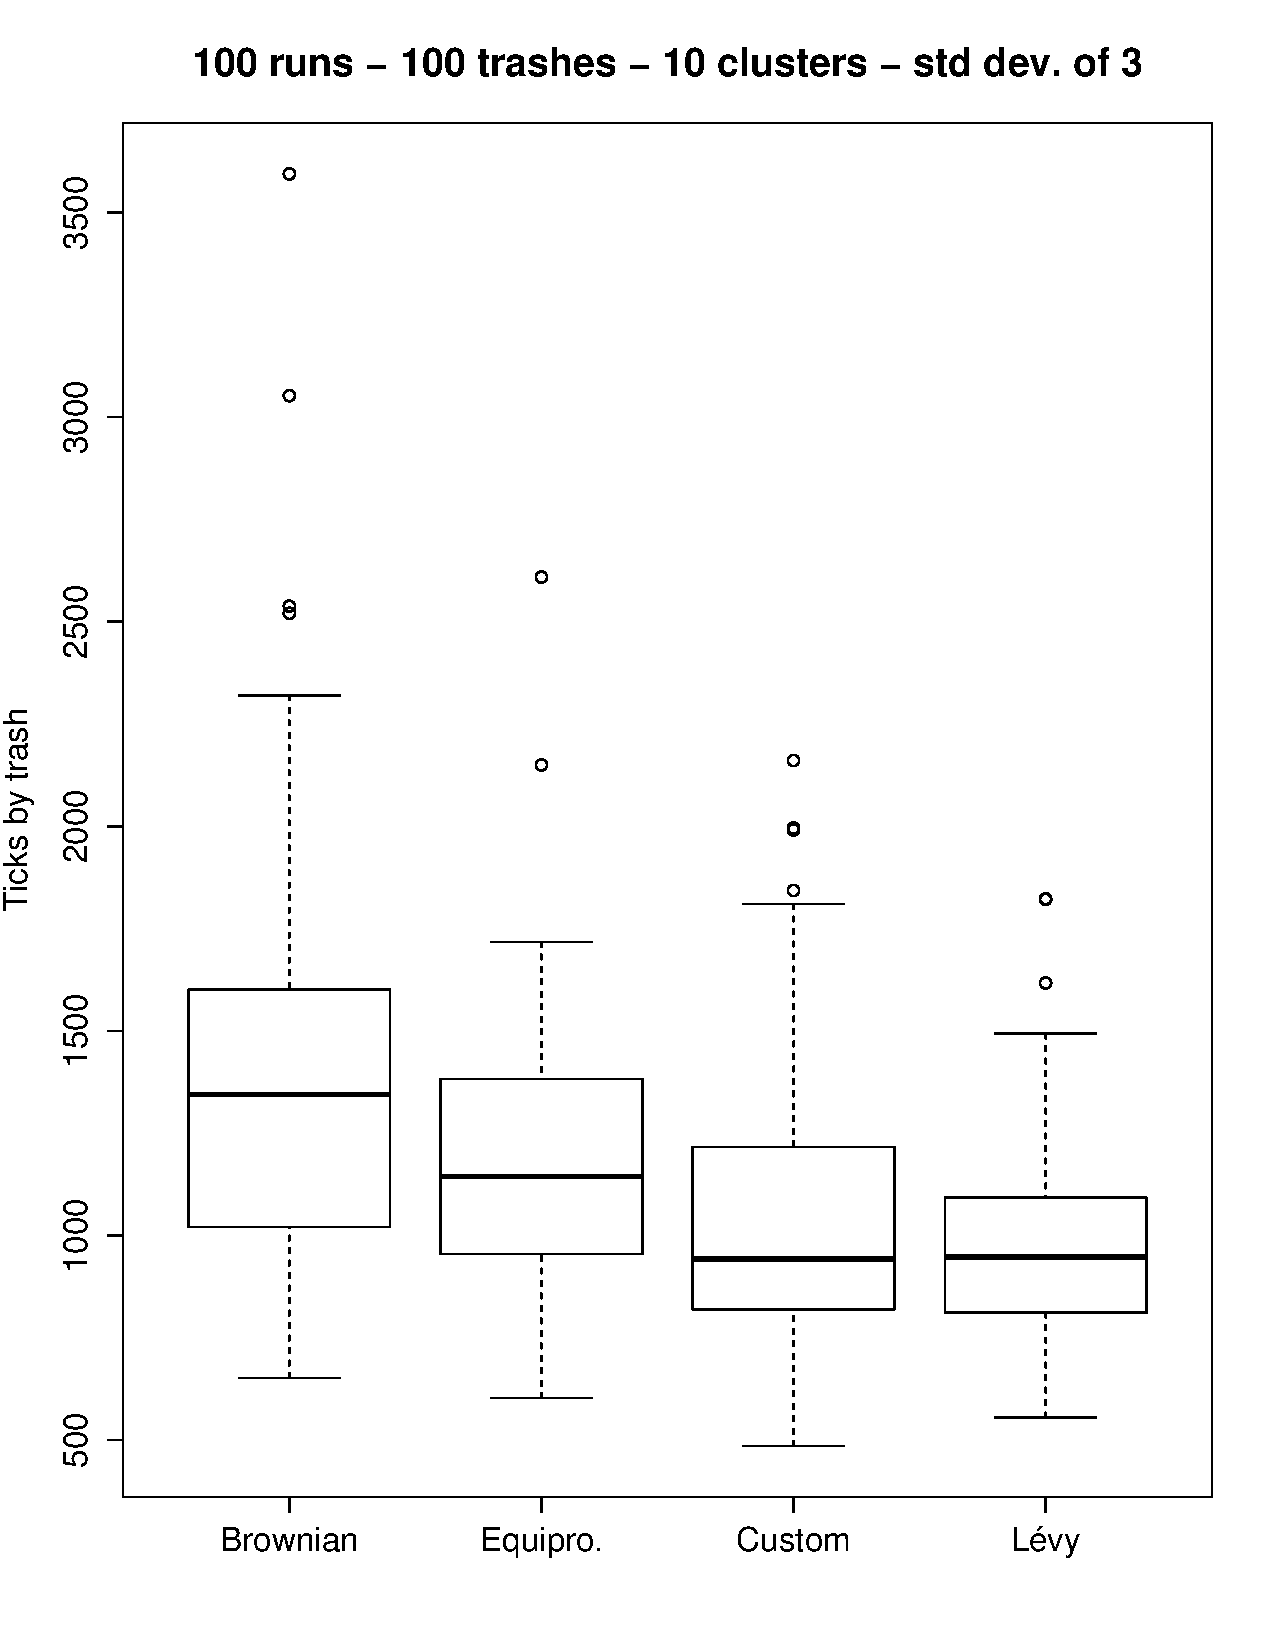
\includegraphics[height=10cm]{diagrams/100Tr10Clts_all.pdf}
		\caption{Résultat des mesures pour 100 débris distribué en 10 clusters (écart-type 3)}
		\label{fig:100Trashes_10Clusters}
	\end{center}
\end{figure}

Nous avons pour les différentes stratégies les statistiques suivantes :

\begin{figure}[H]
	\begin{center}
		\begin{tabular}{| c || c | c | c | c | }
			\hline
			&Brown.&Equi.&Custom&Lévy \\
			\hline
			\hline
			md&1344&1144&942&947\\
			mean&1388&1187&1053&984\\
			min & 652 & 602 & 485 & 555 \\
			max & 3595 & 2609 & 2161 & 1823 \\
			sd&491&318&344&256\\
			p-val&$\ll 5\%$&$\ll 5\%$&$\ll 5\%$&$\ll 5\%$\\
			\hline
		\end{tabular}
		\caption{Statistiques pour 100 débris distribué en 10 clusters (écart-type 3)}
	\end{center}
\end{figure}


Nous pouvons constater que la stratégie Custom a une médiane très
légèrement meilleure à la stratégie Lévy, néanmoins cette première
est moins fiable, c'est à dire que celle-ci a plus de chance de produire
des résultats bien moins bons que le Lévy.

Nous pouvons aussi voir que la stratégie Custom perd en fiabilité
alors que la stratégie Equiprobable, elle, en gagne.
%!TEX root = ../Compte-rendu.tex
\section{Conclusion}

Après différentes mesures pour les quatre stratégies : Brownian,
\'{E}quiprobable, Custom et Lévy, nous pouvons en déduire que celles-ci
ont des performances allant du simple au double. En effet, la
stratégie Brownian est celle qui présente les pires résultats,
alors que la stratégie Lévy est celle qui donne les meilleurs
résultats. La stratégie Custom est globalement meilleure par
rapport à la \'{E}quiprobable, mais nous pouvons constater que l'\'{E}quiprobable
donne des résultats plus proches du Brownian, et la Custom donne
des résultats plus proches du Lévy. Ce résultat s'explique par le
fait que la stratégie \'{E}quiprobable est dérivée du Brownian et
que la Custom est une version modifiée du Lévy.

\end{multicols*}
\end{document}